% Created 2022-10-12 Wed 19:30
% Intended LaTeX compiler: pdflatex
\documentclass[a4paper,11pt,twoside]{article}
\usepackage[utf8]{inputenc}
\usepackage[T1]{fontenc}
\usepackage{graphicx}
\usepackage{longtable}
\usepackage{wrapfig}
\usepackage{rotating}
\usepackage[normalem]{ulem}
\usepackage{amsmath}
\usepackage{amssymb}
\usepackage{capt-of}
\usepackage{hyperref}
\usepackage{minted}
\usepackage{booktabs}
\usepackage{xcolor}
\usepackage{colortbl}
\usepackage{siunitx}
\usepackage{tabu}
\usepackage{etoolbox}
\usepackage{pdflscape}
\usepackage{pgfplots}
\usepackage{tikz}
\usepackage{nopageno}
\usepackage{amssymb}
\usepackage[margin=0.5in]{geometry}
\author{Adityan S}
\date{}
\title{PHN311 Assignment 4}
\hypersetup{
 pdfauthor={Adityan S},
 pdftitle={PHN311 Assignment 4},
 pdfkeywords={},
 pdfsubject={},
 pdfcreator={Emacs 28.2 (Org mode 9.5.5)}, 
 pdflang={English}}
\begin{document}

\maketitle
\tableofcontents

\clearpage

\section{Occilation}
\label{sec:org0e153b7}
Consider the one-dimensional motion of a particle of mass \(m\) in a time independent potential \(V(x)\).Since the energy \(E\) is conserved, one can integrate the equation of motion and obtain a solution in a closed form.

$$
t-C = \sqrt{\frac{m}{2}}\int_{x_i}^x \frac{dx}{\sqrt{E-V(x)}}
$$

For the choice \(C=0\) , the particle is at the position \(x_i\) at the time \(t = 0\) and \(x\) refers to its position at any arbitrary time \(t\). Consider a particular case where the particle is in bound motion between twopoints \(a\) and \(b\) where \(V(x) = E\) for \(x = a, b\) and \(V(x) < E\) for \(a < x < b\). The time period of theoscillation \(T\) is given by,

$$
T = 2 \sqrt{\frac{m}{2}}\int_a^b \frac{dx}{\sqrt{E-V(x)}}
$$

\begin{center}
\includegraphics[width=.9\linewidth]{./ltximg/potwell.png}
\end{center}


\subsection{First consider a particle with \(m = 1 kg\) in the potential \(V(x) = 0.5 \alpha x^2\) with \(\alpha =4 kg sec^2\). Numerically calculate the time period of oscillation and check this against the expected value. Verify that the frequency does not depend on the amplitude of oscillation.}
\label{sec:orgc713963}


\begin{center}
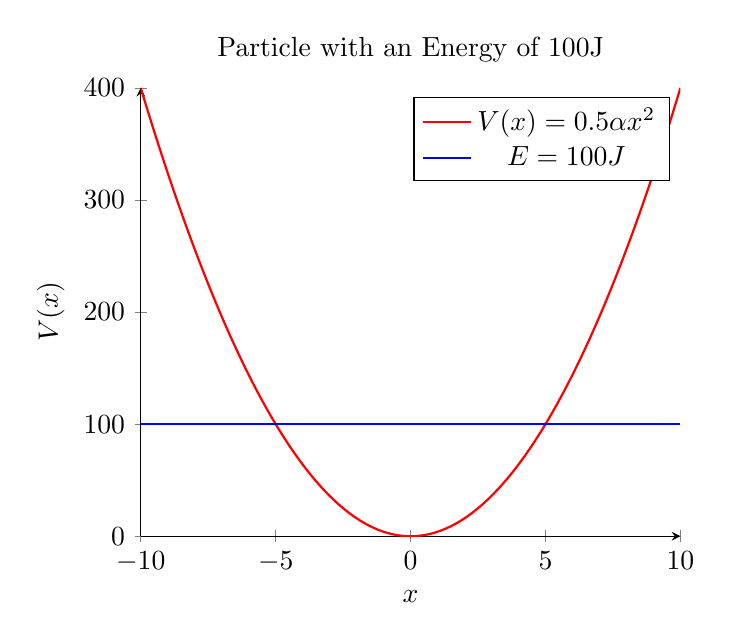
\begin{tikzpicture}
\begin{axis}[title={Particle with an Energy of 100J}, axis lines=left, xlabel=$x$, ylabel=$V(x)$]
\addplot[domain=-10:10, samples=200, thick, red] {4*x^2};
\addlegendentry{$V(x)=0.5\alpha x^2$};
\addplot[domain=-10:10, samples=200, thick, blue] {100};
\addlegendentry{$E = 100J$};
\end{axis}
\end{tikzpicture}
\end{center}

From the above plot, we infer that the for a value of Energy \(E\), the particle is bound for specifc values of \(a\) and \(b\) (decided by \(E\)).

$$
E = V(a)=V(b) = 2x^2
$$

$$
 \implies a = -\sqrt{\frac{E}{2}} = -\frac{A}{\sqrt{2}}, \quad b = +\sqrt{\frac{E}{2}} = +\frac{A}{\sqrt{2}}
$$

Hence Amplitude of occilation is a function of Energy.

$$
A(E) = b-a = \sqrt{E}
$$


\clearpage

From the above equations, the alalytic solution,


$$
T = \sqrt{2}\int_{-\frac{A}{\sqrt{2}}}^{+\frac{A}{\sqrt{2}}} \frac{dx}{\sqrt{A^2-2x^2}} = sin^{-1}{\Big(\frac{\sqrt{2}x}{A}\Big)} \Big|_{-\frac{A}{\sqrt{2}}}^{+\frac{A}{\sqrt{2}}} = \pi \quad (sec)
$$

Using integral identities,  \(T\) can be written as,

$$
T = \sqrt{2}\int_{- \frac{A}{\sqrt2}}^{+ \frac{A}{\sqrt2}} \frac{dx}{\sqrt{A^2-2x^2}}
$$

Let us solve the above numerically for different Amplitudes,

\begin{minted}[breaklines=true,breakanywhere=true]{f90}
program occilation1
  use mods
  real(dp) :: A(200), T(200), xi(6), wi(6), f, x
  f(x) = x**2
  call gauss_legendre(xi, wi)
  integ = sum(wi*f(xi))
  call linspace(-10._dp, 10._dp, A)
  print *, integ
end program occilation1
\end{minted}

\begin{minted}[breaklines=true,breakanywhere=true]{sh}
make occilation1
\end{minted}

\clearpage

\section{Modules}
\label{sec:orgb28e08b}

Module \texttt{mods} consists of all subroutines, variables and procedures that are used in this report. The codeblocks below are all part of the file \texttt{mods.f90}

\begin{minted}[breaklines=true,breakanywhere=true]{f90}
module mods
  use, intrinsic :: iso_fortran_env, only: dp => real64
  use stdlib_quadrature, only: gauss_legendre
  implicit none
  contains
\end{minted}

Linspace Subroutine for creating an array(sequence) with the equal step value.

\begin{minted}[breaklines=true,breakanywhere=true]{f90}
subroutine linspace(from, to, array)
  real(dp), intent(in) :: from, to
  real(dp), intent(out) :: array(:)
  real(dp) :: range
  integer :: n, i
  n = size(array)
  range = to - from
  if (n == 0) return
  if (n == 1) then
     array(1) = from
     return
  end if
  do i=1, n
     array(i) = from + range * (i - 1) / (n - 1)
  end do
end subroutine linspace
\end{minted}

N-point Gauss Legendre Quadrature


\begin{minted}[breaklines=true,breakanywhere=true]{f90}
!working method using stdlib_quadrature

!integer, parameter :: N
!real(dp), dimension(N) :: x, w
!call gauss_legendre(x, w)
!integ = sum(w*f(x))
\end{minted}

End of module \texttt{mods}

\begin{minted}[breaklines=true,breakanywhere=true]{f90}
end module mods
\end{minted}


\clearpage

\section{Makefile}
\label{sec:org801ff69}
\end{document}